% arXiv-style preprint: the basic building blocks of Lemma 3.1.
% Build with a Unicode engine (arXiv supports both):
%   tectonic  lemma31-blocks.tex
%   xelatex   lemma31-blocks.tex   (run twice for references)
% The Lean snippets keep their real unicode, rendered with a unicode mono font.
\documentclass[11pt]{article}

\usepackage[margin=1.25in]{geometry}
\usepackage{amsmath,amssymb}
\usepackage{xcolor}
\usepackage{fontspec}
\usepackage{listings}
\usepackage{tikz}
\usepackage{tikz-cd}
\usetikzlibrary{positioning,arrows.meta,fit,backgrounds}

\usepackage{parskip}          % whitespace between paragraphs
\setlength{\parskip}{1.0em}
\linespread{1.13}

% A unicode monospace font so Lean glyphs (ℕ, →, ≠, ∀, ∑, ...) render directly.
\newfontfamily\leanmono{DejaVu Sans Mono}[Scale=0.82]

% --- a light Lean style for listings -----------------------------------------
\definecolor{leanbg}{gray}{0.97}
\definecolor{leankw}{rgb}{0.30,0.20,0.65}
\definecolor{leancm}{rgb}{0.35,0.45,0.35}
\lstdefinestyle{lean}{
  backgroundcolor=\color{leanbg},
  basicstyle=\leanmono\small,
  keywordstyle=\color{leankw}\bfseries,
  commentstyle=\color{leancm}\itshape,
  morekeywords={def,theorem,lemma,structure,where,fun,Prop,Type,
    instance,variable,namespace,end,open,noncomputable,by,intro,exact,
    show,rw,simp,constructor,have,obtain,Field,Algebra,Function,
    Injective,Bijective,Surjective,LinearMap,import},
  morecomment=[l]{--},
  columns=fullflexible,
  keepspaces=true,
  showstringspaces=false,
  frame=single,
  framesep=6pt,
  xleftmargin=4pt,
  aboveskip=1.1em, belowskip=1.1em,
  extendedchars=true,
}
\lstset{style=lean}
% ------------------------------------------------------------------------------

\title{\bf Inside \texttt{Lemma31.lean}\\[3pt]
  \large A Picture Book of One Clean Trick}
\author{}
\date{}

\begin{document}
\maketitle

\begin{abstract}\noindent
This note opens up one file: \texttt{Lemma31.lean}.

It proves \textbf{Lemma 3.1} of Dempwolff \& M\"uller.
The lemma says:
\[
  x \mapsto L(x)\cdot M(x)\ \text{injective}
  \quad\Longleftrightarrow\quad
  x \mapsto L^{*}(x)\cdot M^{-1}(x)\ \text{injective}.
\]

Here $L$ is linear, $M$ is multiplicative, and $L^{*}$ is the
\emph{trace-adjoint} of $L$.

We walk through every block in the file.
Each block gets a small picture, the matching Lean snippet, and the
Mathlib pieces it leans on.
The English is kept plain on purpose.
\end{abstract}

\bigskip

% =====================================================================
\section{The shape of the file}

The file builds one big equivalence out of small steps.

The pieces, bottom to top:

\begin{itemize}
  \item \texttt{PMap31} --- the product map $P = L\cdot M$.
  \item \texttt{Delta} --- a linear ``twist'' map $\Delta_y$.
  \item \texttt{mul\_map\_zero}, \texttt{mul\_map\_ne\_zero} --- $M$ behaves at $0$.
  \item \texttt{PMap31\_mul\_eq} --- factor $P(xy)$ through $\Delta_y$.
  \item \texttt{PMap31\_inj\_iff\_Delta\_sub\_bij} --- product injective $\Leftrightarrow$ differences bijective.
  \item \texttt{bijective\_iff\_adjoint\_bijective} --- a map is bijective $\Leftrightarrow$ its adjoint is.
  \item \texttt{Delta\_adjoint\_spec} --- the adjoint of $\Delta$ is again a $\Delta$.
  \item \texttt{forall\_ne\_bij} --- relabel ``for all $y_1\neq y_2$'' through a bijection.
  \item \texttt{lemma\_3\_1} --- glue the pieces into the final equivalence.
\end{itemize}

\begin{center}
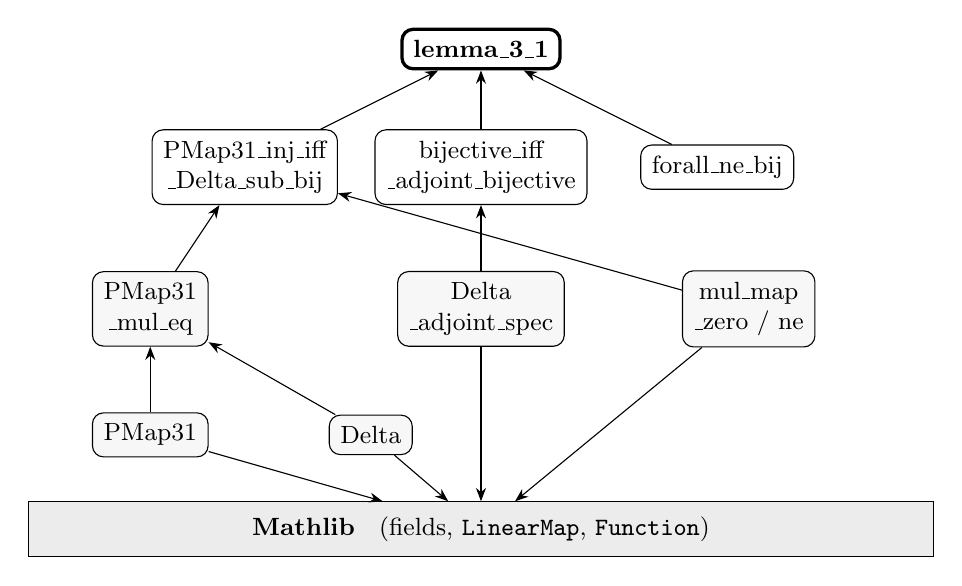
\begin{tikzpicture}[
  every node/.style={font=\small},
  box/.style={draw,rounded corners,align=center,inner sep=4pt,fill=white},
  leaf/.style={draw,rounded corners,align=center,inner sep=4pt,fill=leanbg},
  >=Stealth
]
  \node[box,very thick] (top) at (0,4.0) {\textbf{lemma\_3\_1}};

  \node[box] (inj) at (-3.0,2.5) {PMap31\_inj\_iff\\ \_Delta\_sub\_bij};
  \node[box] (adj) at ( 0.0,2.5) {bijective\_iff\\ \_adjoint\_bijective};
  \node[box] (fab) at ( 3.0,2.5) {forall\_ne\_bij};

  \node[leaf] (mul) at (-4.2,0.7) {PMap31\\ \_mul\_eq};
  \node[leaf] (das) at ( 0.0,0.7) {Delta\\ \_adjoint\_spec};
  \node[leaf] (mz)  at ( 3.4,0.7) {mul\_map\\ \_zero / ne};

  \node[leaf] (pm)  at (-4.2,-0.9) {PMap31};
  \node[leaf] (dl)  at (-1.4,-0.9) {Delta};

  \node[draw,fill=gray!15,minimum width=11.5cm,minimum height=0.7cm]
    (ml) at (0,-2.1) {\textbf{Mathlib} \; (fields, \texttt{LinearMap}, \texttt{Function})};

  \draw[->] (inj) -- (top);
  \draw[->] (adj) -- (top);
  \draw[->] (fab) -- (top);
  \draw[->] (mul) -- (inj);
  \draw[->] (pm)  -- (mul);
  \draw[->] (dl)  -- (mul);
  \draw[->] (das) -- (adj);
  \draw[->] (mz)  -- (inj);
  \draw[->] (pm) -- (ml);
  \draw[->] (dl) -- (ml);
  \draw[->] (mz) -- (ml);
  \draw[->] (das) -- (ml);
\end{tikzpicture}
\end{center}

The whole file imports \emph{only} Mathlib.
So every block sits straight on top of Mathlib.

The setting is fixed once for the file:

\begin{lstlisting}
-- RequestProject/FiniteField/Lemma31.lean
variable {K F : Type*} [Field K] [Field F] [Algebra K F]
         [FiniteDimensional K F] [Finite F]
\end{lstlisting}

\textbf{Mathlib blocks here:}
\begin{itemize}
  \item \texttt{Field} --- $K$ and $F$ are fields.
  \item \texttt{Algebra K F} --- $F$ is a vector space (and algebra) over $K$.
  \item \texttt{FiniteDimensional}, \texttt{Finite} --- so injective $=$ surjective.
\end{itemize}

% =====================================================================
\section{Block 1 --- \texttt{PMap31}: the product map}

The whole story is about one map.
Take a linear map $L$ and any map $M$.
Multiply their outputs:
\[
  P(x) \;=\; L(x)\cdot M(x).
\]

\begin{center}
\begin{tikzcd}[column sep=large,row sep=tiny]
  & L(x) \arrow[dr,"\cdot"] & \\
  x \arrow[ur,"L"] \arrow[dr,"M"'] & & L(x)\cdot M(x) \\
  & M(x) \arrow[ur,"\cdot"'] &
\end{tikzcd}
\end{center}

\begin{lstlisting}
def PMap31 (L : F →ₗ[K] F) (M : F → F) (x : F) : F := L x * M x
\end{lstlisting}

\textbf{Mathlib blocks:} the bundled $K$-linear map type \,$F \to_{\ell} F$\,, and field multiplication.

% =====================================================================
\section{Block 2 --- \texttt{Delta}: the twist map}

Now fix a second input $y$.
Twist $x$ by $y$ \emph{before} applying $L$, then scale by $M(y)$:
\[
  \Delta_y(x) \;=\; L(x\cdot y)\cdot M(y).
\]

The key point: for a fixed $y$, this is \textbf{linear in $x$}.
So $\Delta_y$ is a genuine \texttt{LinearMap}.

\begin{center}
\begin{tikzcd}[column sep=huge]
  x \arrow[r,"\cdot\,y"] & x\,y \arrow[r,"L"] & L(x\,y) \arrow[r,"\cdot\,M(y)"] & \Delta_y(x)
\end{tikzcd}
\end{center}

\begin{lstlisting}
noncomputable def Delta (L : F →ₗ[K] F) (M : F → F) (y : F) : F →ₗ[K] F where
  toFun x := L (x * y) * M y
  map_add' x₁ x₂ := by simp [add_mul, map_add, add_mul]
  map_smul' r x := by
    show L ((r • x) * y) * M y = r • (L (x * y) * M y)
    rw [smul_mul_assoc, map_smul, smul_mul_assoc]

@[simp] lemma Delta_apply (L : F →ₗ[K] F) (M : F → F) (y x : F) :
    Delta L M y x = L (x * y) * M y := rfl
\end{lstlisting}

\textbf{Proof steps:}
\begin{itemize}
  \item \texttt{map\_add'}: opens $(x_1+x_2)y$ with \texttt{add\_mul}, then $L$
        is additive (\texttt{map\_add}).
  \item \texttt{map\_smul'}: scalars slide out with \texttt{smul\_mul\_assoc}
        and $L$ is linear (\texttt{map\_smul}).
  \item \texttt{Delta\_apply}: holds by \texttt{rfl} (just unfolding).
\end{itemize}

\textbf{Mathlib blocks:} \texttt{add\_mul}, \texttt{map\_add},
\texttt{map\_smul}, \texttt{smul\_mul\_assoc}, and the \texttt{LinearMap}
bundle (\texttt{toFun}, \texttt{map\_add'}, \texttt{map\_smul'}).

% =====================================================================
\section{Block 3 --- \texttt{M} behaves at zero}

We need two tiny facts about a multiplicative, injective $M$.

\begin{itemize}
  \item If $M(ab)=M(a)M(b)$ and $M$ is injective, then $M(0)=0$.
  \item Then $M$ sends nonzero to nonzero.
\end{itemize}

Why $M(0)=0$?
If not, then $M(0)=M(0)M(x)$ forces $M(x)=1$ for \emph{every} $x$.
That kills injectivity.  Contradiction.

\begin{center}
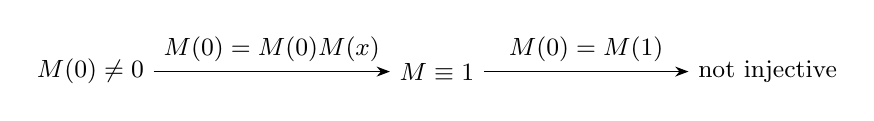
\begin{tikzpicture}[every node/.style={font=\small},>=Stealth]
  \node (a) at (0,0) {$M(0)\neq 0$};
  \node (b) at (4.4,0) {$M\equiv 1$};
  \node (c) at (8.6,0) {not injective};
  \draw[->] (a) -- node[above]{$M(0)=M(0)M(x)$} (b);
  \draw[->] (b) -- node[above]{$M(0)=M(1)$} (c);
\end{tikzpicture}
\end{center}

\begin{lstlisting}
lemma mul_map_zero {M : F' → F'} (hM : ∀ a b, M (a * b) = M a * M b)
    (hMinj : Function.Injective M) : M 0 = 0 := by
  by_contra h
  have hM0 : ∀ x : F', M x = 1 := by intro x; specialize hM 0 x; aesop
  simpa [hM0] using @hMinj 0 1

lemma mul_map_ne_zero {M : F' → F'} (hMinj : Function.Injective M)
    (hM0 : M 0 = 0) {x : F'} (hx : x ≠ 0) : M x ≠ 0 :=
  fun h => hx (hMinj (h.trans hM0.symm))
\end{lstlisting}

\textbf{Proof steps:} \texttt{by\_contra}, then \texttt{aesop} closes the
``$M\equiv 1$'' step; \texttt{simpa} hits injectivity at $0$ vs $1$.

\textbf{Mathlib blocks:} \texttt{Function.Injective},
\texttt{by\_contra}, \texttt{aesop}, \texttt{Eq.trans}.

% =====================================================================
\section{Block 4 --- \texttt{PMap31\_mul\_eq}: factor the product}

This is the bridge between $P$ and $\Delta$.

Feed $P$ the product $x\cdot y$.  Then it splits:
\[
  P(x\,y) \;=\; \Delta_y(x)\cdot M(x).
\]

So the product map, evaluated on $xy$, is the twist map times $M(x)$.

\begin{center}
\begin{tikzcd}[column sep=2.2cm]
  P(x\,y) \arrow[r,equal] & \Delta_y(x)\,\cdot\,M(x)
\end{tikzcd}
\end{center}

\begin{lstlisting}
lemma PMap31_mul_eq (L : F →ₗ[K] F) {M : F → F}
    (hM : ∀ a b, M (a * b) = M a * M b) (x y : F) :
    PMap31 L M (x * y) = Delta L M y x * M x := by
  simp [PMap31, hM]; ring
\end{lstlisting}

\textbf{Proof steps:} unfold \texttt{PMap31}, split $M(xy)=M(x)M(y)$ with
\texttt{hM}, then \texttt{ring} rearranges the product.

\textbf{Mathlib blocks:} \texttt{simp}, \texttt{ring}.

% =====================================================================
\section{Block 5 --- product injective $\Leftrightarrow$ differences bijective}

This is the heart of the file.

\textbf{Claim.} $P$ is injective exactly when, for every $y_1\neq y_2$, the
difference of twist maps
\[
  \Delta_{y_1} - \Delta_{y_2}
\]
is bijective.

\begin{center}
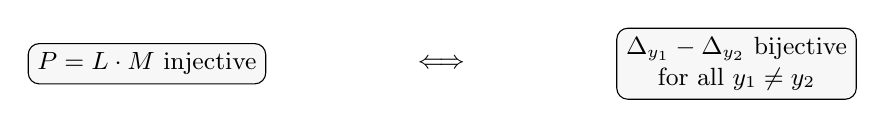
\begin{tikzpicture}[every node/.style={font=\small},>=Stealth,node distance=10mm]
  \node[draw,rounded corners,fill=leanbg] (p) {$P=L\cdot M$ injective};
  \node[right=18mm of p] (mid) {$\Longleftrightarrow$};
  \node[draw,rounded corners,fill=leanbg,align=center,right=18mm of mid] (d)
    {$\Delta_{y_1}-\Delta_{y_2}$ bijective\\ for all $y_1\neq y_2$};
\end{tikzpicture}
\end{center}

Why it works, in one breath:
$P(xy_1)=P(xy_2)$ becomes $(\Delta_{y_1}-\Delta_{y_2})(x)=0$ after the factor
trick (Block~4).  So ``no collisions'' for $P$ means ``trivial kernel'' for the
difference --- i.e.\ injective, hence bijective in finite dimension.

\begin{lstlisting}
lemma PMap31_inj_iff_Delta_sub_bij (L : F →ₗ[K] F) {M : F → F}
    (hM : ∀ a b, M (a * b) = M a * M b) (hMinj : Function.Injective M) :
    Function.Injective (PMap31 L M) ↔
    ∀ y₁ y₂ : F, y₁ ≠ y₂ → Function.Bijective (Delta L M y₁ - Delta L M y₂)
\end{lstlisting}

\textbf{Proof steps:}
\begin{itemize}
  \item ($\Rightarrow$) From a kernel vector $x$, build
        $P(xy_1)=P(xy_2)$, apply injectivity, get $x=0$;
        so the kernel is trivial.
  \item Trivial kernel $\Rightarrow$ injective via
        \texttt{LinearMap.ker\_eq\_bot}; then injective $\Rightarrow$
        surjective via \texttt{LinearMap.surjective\_of\_injective}.
  \item ($\Leftarrow$) If $P$ collides at $x,y$ with $x\neq y$, the
        difference map kills $1$, contradicting bijectivity.
\end{itemize}

\textbf{Mathlib blocks:}
\texttt{LinearMap.ker\_eq\_bot}, \texttt{LinearMap.ker\_eq\_bot'},
\texttt{LinearMap.surjective\_of\_injective}, \texttt{Function.Bijective}.

% =====================================================================
\section{Block 6 --- a map is bijective iff its adjoint is}

Now bring in a nondegenerate \emph{trace form} $T : F \to K$.
``Nondegenerate'' means: if $T(xy)=0$ for all $y$, then $x=0$.

Suppose $A$ and $A^{*}$ are adjoint with respect to $T$:
\[
  T(A u \cdot v) \;=\; T(u \cdot A^{*} v) \qquad \text{for all } u,v.
\]

Then $A$ is bijective \emph{iff} $A^{*}$ is bijective.

\[
  T\bigl(A u \cdot v\bigr) \;=\; T\bigl(u \cdot A^{*} v\bigr)
  \qquad\Longrightarrow\qquad
  \bigl(A\ \text{bijective}\bigr) \Leftrightarrow \bigl(A^{*}\ \text{bijective}\bigr).
\]

\begin{lstlisting}
lemma bijective_iff_adjoint_bijective (T : F →ₗ[K] K)
    (hT : ∀ x : F, (∀ y : F, T (x * y) = 0) → x = 0)
    (A Aadj : F →ₗ[K] F)
    (hAdj : ∀ u v, T (A u * v) = T (u * Aadj v)) :
    Function.Bijective A ↔ Function.Bijective Aadj
\end{lstlisting}

\textbf{Proof steps:}
\begin{itemize}
  \item One direction: surjectivity of $A$ plus the pairing makes $T(\cdot,\,)$
        nondegenerate enough to force $A^{*}$ injective.
  \item Injective $\Rightarrow$ bijective by finiteness
        (\texttt{Finite.injective\_iff\_surjective}).
  \item The reverse direction is the mirror image.
\end{itemize}

\textbf{Mathlib blocks:}
\texttt{sub\_eq\_zero}, \texttt{mul\_sub}, \texttt{sub\_mul},
\texttt{Finite.injective\_iff\_surjective},
\texttt{LinearMap.surjective\_of\_injective}.

% =====================================================================
\section{Block 7 --- the adjoint of a twist is a twist}

We need the adjoint of $\Delta$ to stay in the same family.

With $L^{*}$ the adjoint of $L$ and $M^{-1}$ the inverse of $M$:
\[
  T\bigl(\Delta_y^{L,M}(u)\cdot v\bigr)
  \;=\;
  T\bigl(u\cdot \Delta_{M(y)}^{\,L^{*},M^{-1}}(v)\bigr).
\]

So the adjoint of ``twist by $y$ with $(L,M)$'' is again a twist ---
now ``twist by $M(y)$ with $(L^{*},M^{-1})$''.
The family is closed under adjoints.

\begin{center}
\begin{tikzcd}[column sep=1.6cm]
  \Delta^{L,M}_{y} \arrow[r,"\text{adjoint}"] & \Delta^{L^{*},M^{-1}}_{M(y)}
\end{tikzcd}
\end{center}

\begin{lstlisting}
lemma Delta_adjoint_spec (T : F →ₗ[K] K) (L Ladj : F →ₗ[K] F)
    (hAdj : ∀ w z, T (L w * z) = T (w * Ladj z))
    {M Minv : F → F} (hMinv : ∀ x, Minv (M x) = x)
    (u v y : F) :
    T (Delta L M y u * v) = T (u * Delta Ladj Minv (M y) v) := by
  have := hAdj (u * y) (v * M y)
  simp_all +decide [mul_assoc, mul_left_comm]
  convert this using 1 <;> ring
\end{lstlisting}

\textbf{Proof steps:} feed the $L$/$L^{*}$ adjoint rule the points
$(uy,\, v\,M(y))$, simplify the products, then \texttt{ring} matches both
sides.

\textbf{Mathlib blocks:} \texttt{mul\_assoc}, \texttt{mul\_left\_comm},
\texttt{convert}, \texttt{ring}, \texttt{simp\_all}.

% =====================================================================
\section{Block 8 --- relabel ``for all $y_1\neq y_2$''}

A small combinatorial step.

We have a property $Q$ stated for all pairs $M(y_1)\neq M(y_2)$.
Since $M$ is a bijection, this is the same as $Q$ for all pairs
$z_1\neq z_2$.

In words: a bijection just \emph{renames} the elements, so a
``for all distinct pairs'' statement is unchanged.

\begin{center}
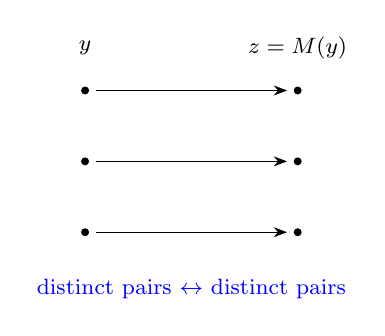
\begin{tikzpicture}[scale=0.9,>=Stealth,every node/.style={font=\footnotesize}]
  % left column y's, right column z=M(y), pairs preserved
  \foreach \i in {0,1,2} {
    \fill (0,-\i) circle (1.6pt);
    \fill (3,-\i) circle (1.6pt);
    \draw[->] (0.15,-\i) -- (2.85,-\i);
  }
  \node at (0,0.6) {$y$};
  \node at (3,0.6) {$z=M(y)$};
  \node[blue] at (1.5,-2.8) {distinct pairs $\leftrightarrow$ distinct pairs};
\end{tikzpicture}
\end{center}

\begin{lstlisting}
lemma forall_ne_bij {α : Type*} {M : α → α} (hMbij : Function.Bijective M)
    {Q : α → α → Prop} :
    (∀ y₁ y₂, y₁ ≠ y₂ → Q (M y₁) (M y₂)) ↔ (∀ z₁ z₂, z₁ ≠ z₂ → Q z₁ z₂) := by
  constructor <;> intro h z₁ z₂ hz
  · obtain ⟨y₁, rfl⟩ := hMbij.2 z₁
    obtain ⟨y₂, rfl⟩ := hMbij.2 z₂
    exact h y₁ y₂ (fun heq => hz (congr_arg M heq))
  · exact h _ _ (fun heq => hz (hMbij.1 heq))
\end{lstlisting}

\textbf{Proof steps:} pull preimages with surjectivity (\texttt{hMbij.2}); keep
distinctness with injectivity (\texttt{hMbij.1}).

\textbf{Mathlib blocks:} \texttt{Function.Bijective},
\texttt{congr\_arg}.

% =====================================================================
\section{Block 9 --- \texttt{lemma\_3\_1}: glue it all}

Finally, put the blocks together.

\textbf{Lemma 3.1.}
\[
  L(x)\cdot M(x)\ \text{injective}
  \quad\Longleftrightarrow\quad
  L^{*}(x)\cdot M^{-1}(x)\ \text{injective}.
\]

The chain of rewrites:

\begin{enumerate}
  \item Rewrite \emph{both} sides with Block~5
        (\texttt{PMap31\_inj\_iff\_Delta\_sub\_bij}):\\
        each side becomes ``all differences bijective''.
  \item For each pair $y_1,y_2$, use Block~6
        (\texttt{bijective\_iff\_adjoint\_bijective}) with the adjoint
        from Block~7 (\texttt{Delta\_adjoint\_spec}):\\
        the $(L,M)$ difference is bijective iff the
        $(L^{*},M^{-1})$ difference is.
  \item The right side ranges over $M(y_1)\neq M(y_2)$.
        Block~8 (\texttt{forall\_ne\_bij}) relabels it to all $z_1\neq z_2$.
\end{enumerate}

\begin{center}
\begin{tikzcd}[column sep=1.5cm,row sep=large]
  L\cdot M\ \text{inj}
    \arrow[r,"\text{Block 5}"] &
  \Delta^{L,M}\ \text{bij}
    \arrow[r,"\text{Blocks 6,7}"] &
  \Delta^{L^{*},M^{-1}}\ \text{bij}
    \arrow[r,"\text{Block 8}"] &
  L^{*}\cdot M^{-1}\ \text{inj}
\end{tikzcd}
\end{center}

\begin{lstlisting}
theorem lemma_3_1 (T : F →ₗ[K] K)
    (hT : ∀ x : F, (∀ y : F, T (x * y) = 0) → x = 0)
    (L Ladj : F →ₗ[K] F)
    (hAdj : ∀ w z, T (L w * z) = T (w * Ladj z))
    (M Minv : F → F)
    (hM_mul : ∀ a b, M (a * b) = M a * M b)
    (hM_bij : Function.Bijective M)
    (hMinv_mul : ∀ a b, Minv (a * b) = Minv a * Minv b)
    (hMinv_inj : Function.Injective Minv)
    (hMinvL : ∀ x, Minv (M x) = x)
    (hMinvR : ∀ x, M (Minv x) = x) :
    Function.Injective (PMap31 L M) ↔ Function.Injective (PMap31 Ladj Minv) := by
  rw [PMap31_inj_iff_Delta_sub_bij L hM_mul hM_bij.injective]
  rw [PMap31_inj_iff_Delta_sub_bij Ladj hMinv_mul hMinv_inj]
  have h_bijective_iff_adjoint_bijective :
      ∀ y₁ y₂ : F, Function.Bijective (Delta L M y₁ - Delta L M y₂) ↔
        Function.Bijective (Delta Ladj Minv (M y₁) - Delta Ladj Minv (M y₂)) := by
    intro y₁ y₂
    apply bijective_iff_adjoint_bijective T hT
    intro u v; simp +decide [Delta, hAdj]; ring
    simp +decide [mul_assoc, hAdj, hMinvL]
    simp +decide only [mul_comm]
  convert forall_ne_bij hM_bij using 1
  simp +decide only [h_bijective_iff_adjoint_bijective]
\end{lstlisting}

\textbf{Mathlib blocks:} \texttt{rw}, \texttt{convert}, \texttt{simp},
\texttt{ring}, plus the file's own Blocks 5--8.

% =====================================================================
\section{One sentence to remember}

\texttt{Lemma31.lean} swaps a hard \emph{product} question for an easy
\emph{linear} one --- and a trace adjoint flips the linear map and inverts the
multiplier, leaving injectivity untouched.

\bigskip
\begin{center}\small
Two maps, one twist, one adjoint, one equivalence.
\end{center}

\end{document}
